% diagrams/english/patio.tex -- el patio de la casa de la abuela, en el
% pueblo, para "Where is it?": de izquierda a derecha, el gallinero (con
% su tejado a dos aguas), el limonero, la mesa, el banco, la pila de
% piedra con su grifo y la tapia. Es el mismo patio que el mapa del día
% 241: el gallinero a la izquierda, el limonero en el medio y la mesa con
% el banco a la derecha.
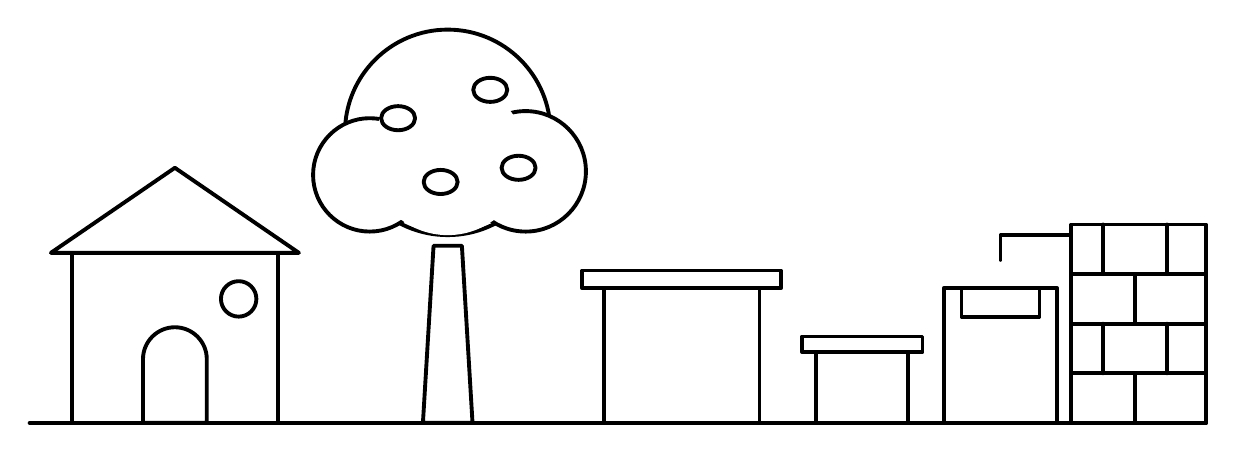
\begin{tikzpicture}[line width=1.4pt, line cap=round, line join=round, scale=0.9]
  \draw (-0.3,0) -- (16.3,0);
  % el gallinero: la caseta, el tejado, la puerta y un ventanuco
  \filldraw[fill=white] (0.3,0) rectangle (3.2,2.4);
  \filldraw[fill=white] (0.0,2.4) -- (1.75,3.6) -- (3.5,2.4) -- cycle;
  \filldraw[fill=white] (1.3,0) -- (1.3,0.9) arc (180:0:0.45) -- (2.2,0) -- cycle;
  \filldraw[fill=white] (2.65,1.75) circle (0.25);
  % el limonero, con cuatro limones en la copa
  \filldraw[fill=white] (5.25,0) -- (5.4,2.5) -- (5.8,2.5) -- (5.95,0) -- cycle;
  \filldraw[fill=white] (5.6,4.1) circle (1.45);
  \filldraw[fill=white] (4.5,3.5) circle (0.8);
  \filldraw[fill=white] (6.7,3.55) circle (0.85);
  \fill[white] (5.6,3.75) circle (1.1);
  \foreach \x/\y in {4.9/4.3, 6.2/4.7, 5.5/3.4, 6.6/3.6} {
    \filldraw[fill=white] (\x,\y) ellipse (0.24 and 0.17);
  }
  % la mesa
  \filldraw[fill=white] (7.5,1.9) rectangle (10.3,2.15);
  \draw (7.8,1.9) -- (7.8,0); \draw (10.0,1.9) -- (10.0,0);
  % el banco
  \filldraw[fill=white] (10.6,1.0) rectangle (12.3,1.22);
  \draw (10.8,1.0) -- (10.8,0); \draw (12.1,1.0) -- (12.1,0);
  % la pila de piedra, con el agua arriba, y el grifo que sale de la tapia
  \filldraw[fill=white] (12.6,0) rectangle (14.2,1.9);
  \draw (12.85,1.9) -- (12.85,1.5) -- (13.95,1.5) -- (13.95,1.9);
  \draw (14.4,2.65) -- (13.4,2.65) -- (13.4,2.3);
  % la tapia de ladrillo
  \filldraw[fill=white] (14.4,0) rectangle (16.3,2.8);
  \foreach \y in {0.7,1.4,2.1} { \draw (14.4,\y) -- (16.3,\y); }
  \foreach \x/\y in {15.3/0, 14.85/0.7, 15.75/0.7, 15.3/1.4, 14.85/2.1, 15.75/2.1} {
    \draw (\x,\y) -- (\x,\y+0.7);
  }
\end{tikzpicture}
